%% Separable mixed-frequency reduction (Figure 2). Compile with pdflatex, then convert to PNG.
\documentclass[border=2pt]{standalone}
\usepackage{amsmath,amssymb}
\usepackage{tikz}
\usetikzlibrary{arrows.meta}
\definecolor{cPol}{HTML}{3B5BA5}
\definecolor{cShr}{HTML}{2E8B57}
\definecolor{cCO}{HTML}{8C5A3C}
\definecolor{cInk}{HTML}{2D3748}
\newcommand{\ifwg}{\mathrm{IFWG}}
\begin{document}
\sffamily
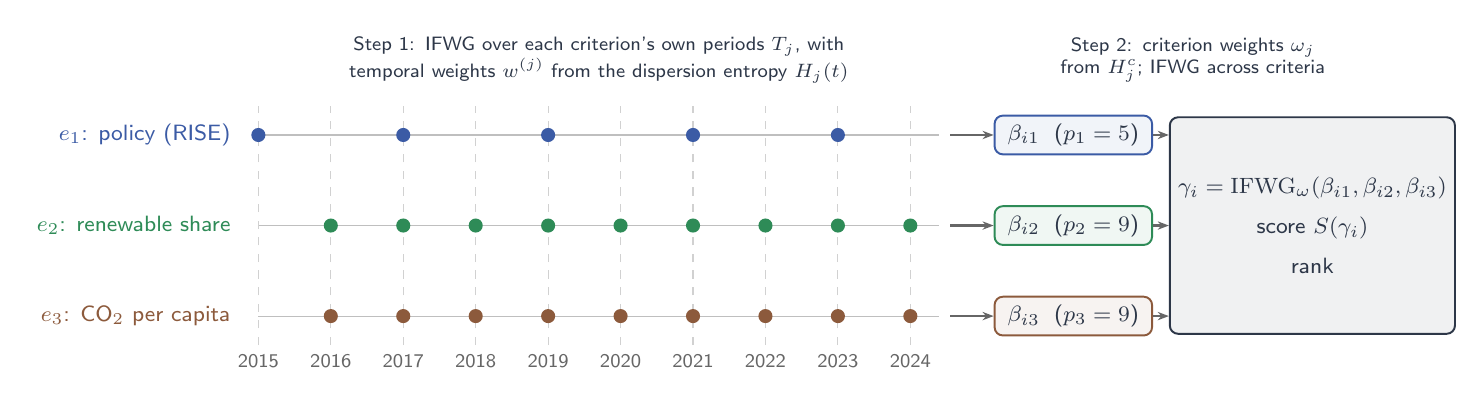
\begin{tikzpicture}[font=\sffamily\footnotesize, text=cInk, x=0.92cm, y=1.15cm,
  obs/.style={circle, fill=#1, inner sep=1.8pt},
  box/.style={draw=#1, fill=#1!7, rounded corners=3pt, align=center, inner sep=3pt, minimum width=2.0cm, line width=0.7pt},
  >={Stealth[length=4pt]}]
  \foreach \y/\lab/\col in {2/{$e_1$: policy (RISE)}/cPol, 1/{$e_2$: renewable share}/cShr, 0/{$e_3$: CO$_2$ per capita}/cCO}{
    \node[anchor=east, text=\col] at (-0.25,\y) {\lab};
    \draw[black!25] (0,\y) -- (9.4,\y);}
  \foreach \x/\yr in {0/2015,1/2016,2/2017,3/2018,4/2019,5/2020,6/2021,7/2022,8/2023,9/2024}{
    \draw[black!18, dashed] (\x,-0.32) -- (\x,2.32); \node[below, font=\sffamily\scriptsize, text=black!60] at (\x,-0.32) {\yr};}
  \foreach \x in {0,2,4,6,8} \node[obs=cPol] at (\x,2) {};
  \foreach \x in {1,...,9} {\node[obs=cShr] at (\x,1) {}; \node[obs=cCO] at (\x,0) {};}
  \node[box=cPol] (r1) at (11.25,2) {$\beta_{i1}$\; ($p_1=5$)};
  \node[box=cShr] (r2) at (11.25,1) {$\beta_{i2}$\; ($p_2=9$)};
  \node[box=cCO]  (r3) at (11.25,0) {$\beta_{i3}$\; ($p_3=9$)};
  \foreach \y/\n in {2/r1,1/r2,0/r3} \draw[->, black!60, line width=0.8pt] (9.55,\y) -- (\n.west);
  \node[box=cInk, minimum width=2.45cm, minimum height=2.75cm] (g) at (14.55,1)
       {$\gamma_i=\ifwg_\omega(\beta_{i1},\beta_{i2},\beta_{i3})$\\[5pt] score $S(\gamma_i)$\\[5pt] rank};
  \foreach \n in {r1,r2,r3} \draw[->, black!60, line width=0.8pt] (\n.east) -- (g.west |- \n.east);
  \node[align=center, font=\sffamily\scriptsize, text width=8.6cm] at (4.7,2.83)
       {Step 1: IFWG over each criterion's own periods $T_j$, with temporal weights $w^{(j)}$ from the dispersion entropy $H_j(t)$};
  \node[align=center, font=\sffamily\scriptsize, text width=5.0cm] at (12.9,2.83)
       {Step 2: criterion weights $\omega_j$ from $H^c_j$; IFWG across criteria};
\end{tikzpicture}
\end{document}
